\documentclass[11pt]{article}

\usepackage[final]{neurips_2019}
\usepackage{amssymb}
\usepackage{amsmath}
\usepackage{hyperref}  %hyperref still needs to be put at the end!
%\usepackage[sorting=none]{biblatex}
%\addbibresource{references.bib}
\usepackage{graphicx}
\usepackage[title]{appendix}

%\usepackage[square,numbers]{natbib}
\bibliographystyle{abbrvnat}


\newcommand{\numpy}{{\tt numpy}}    % tt font for numpy
\DeclareMathOperator*{\argmin}{arg\,min}

%\topmargin -.5in
%\textheight 9in
%\oddsidemargin -.25in
%\evensidemargin -.25in
%\textwidth 7in

\begin{document}


% ========== Edit your name here
\author{Lucas Jaffe \\ PhD Student in Berkeley EECS Department \\ Email: lucasjaffe@berkeley.edu \\ Document date: May 9$^{\textrm{th}}$, 2020}

\title{
    Analysis of Gradient Descent \\ on the Triplet Margin Loss \\
    \large EECS227C Project
    }
\maketitle

\medskip

% In this work we study:
% \begin{itemize}
%     \item Two metric learning objectives
%     \item Relaxation and reformulation of these objectives as DC functions
%     \item Smoothability of these objectives, and study of accuracy/smoothness tradeoff
%     \item Dependence on data of conditioning of the problem
%     \item Study of smoothness parameters vs. minima for original and smooth relaxation
%     \item Interpretations of these objectives as learning a separating hyperplane with soft margin
%     \item Extension of the objectives to learning an affine mapping instead of weight vector
%     \item Different gradient methods for minimization of these objectives
%     \item Possible extensions to the empirical risk minimization setting
% \end{itemize}


% Other stuff:
% \begin{itemize}
%     \item Different learning rate selection including exact line search, backtracking line search
%     \item Nesterov momentum for speedup (for badly conditioned problems?)
% \end{itemize}

\section{Introduction}

% ========== Begin answering questions here 
The goal of this project is to study gradient descent on the triplet margin loss function, a non-convex objective function used in the metric learning domain. The GitHub repository for the project is linked here\footnote{\url{https://github.com/LukeJaffe/eecs227c_project}}.

We show that the triplet margin loss function can be reformulated as a difference of convex functions, and that a reasonable smooth approximation can be formulated with the LogSumExp function. We show that this function is smooth, and give an upper bound for the smoothness which is dependent on the iterate. Then, we show that a descent condition holds for the gradient descent algorithm, given the right choice of stepsize. Finally, we attempt a gradient descent convergence analysis for the iterate, the squared gradient norm, and the function value, and discuss insight from these efforts.

\subsection{Background}
 
 Given some data $X \in \mathbb{R}^{n \times m}$ and corresponding labels $Y \in \mathbb{R}^n$, in the supervised metric learning problem, the goal is to find a mapping $\phi: \mathbb{R}^{n \times m} \rightarrow \mathbb{R}^{n \times d}$, such that samples with the same label are close together in some metric space, and samples with different labels are further apart. Classically, this type of problem formulation was studied as a dimensionality reduction method, as in \cite{hadsell_dimensionality_2006}, or for k-nearest neighbors classification, as in \cite{weinberger_distance_2009}. More recently, metric learning has been combined with deep learning into a highly accurate vehicle for solving a range problems in computer vision and natural language processing. 
 
 %verification, re-identification, and retrieval. In the image verification problem, the goal is to tell whether two images belong to the same instance. This is commonly used for authentication of identity, either for unlocking a smartphone\footnote{\url{https://support.apple.com/en-us/HT208108}}, or more recently for airport security (\cite{mccartney_are_2019}). In the image re-identification problem, the goal is to search a database for a single matching image to a query image. This is commonly used for re-identification of people (\cite{zheng_scalable_2015}) / faces (\cite{schroff_facenet_2015}), and vehicles (\cite{liu_deep_2016}). In the image retrieval problem, the goal is to return all similar or matching images to a query image. This is used in reverse image search applications, e.g., from Google\footnote{\url{https://support.google.com/websearch/answer/1325808?co=GENIE.Platform\%3DDesktop&hl=en}} and new law enforcement applications including the platform developed by ClearView AI\footnote{\url{https://clearview.ai/}}.

\subsection{Problem setup}

The \textit{triplet margin loss} function is a common metric learning objective function, which has been demonstrated as empirically effective in the deep learning literature, esp. for facial recognition \cite{schroff_facenet_2015}. This is the primary objective function used in the popular OpenFace library (\cite{amos_openface_2016}). Further, this objective has longevity in the literature, having been used in \cite{araujo_large_2009}, defended in \cite{hermans_defense_2017}, and recently generalized in \cite{qian_softtriple_2019}.

A triplet is defined as a set of three samples, two of which share the same label, and one of which has a different label. Given some data $X \in \mathbb{R}^{n \times m}$ and corresponding labels $Y \in \mathbb{R}^n$, we define $X' \in \mathbb{R}^{n' \times m}$ as the set of all possible triplets from $X, Y$. For a given triplet $x_i$, we denote the two samples sharing a label as $x_i^a, x_i^p$ (anchor and positive), and the third sample $x_i^n$ (negative). In addition, we define a margin parameter $\alpha \in \mathbb{R}^+$. Then the triplet margin loss can be stated as follows:

\begin{equation}
    \frac{1}{n'} \sum_{i=1}^{n'} \max(0, \| \phi(x_i^a) - \phi(x_i^p)\|_2^2 - \| \phi(x_i^a) - \phi(x_i^n)\|_2^2 + \alpha)
\end{equation}

We note that the triplet margin formulation described here closely follows from \cite{schroff_facenet_2015}.

Observing $\phi$ as a function of some parameter set $\theta$, parameterized by the triplet set $X'$, we can use our objective for empirical risk minimization by solving the following optimization problem:

\begin{equation}
\label{eq:triplet_objective}
\begin{aligned}
    \min_{\theta} \frac{1}{n'} \sum_{i=1}^{n'} \max(0, \| \phi(\theta; x_i^a) - \phi(\theta; x_i^p)\|_2^2 - \| \phi(\theta; x_i^a) - \phi(\theta; x_i^n)\|_2^2 + \alpha)
\end{aligned}
\end{equation}

Conceptually, the goal of this problem is to learn $\theta$ such that samples with the same label are closer together in Euclidean space than samples with different labels. Observing each class cluster as a hypersphere in $\mathbb{R}^d$, achieving a value of $0$ for this objective corresponds to pushing each class hypersphere apart by the max squared diameter of any class hypersphere plus the margin parameter $\alpha$. In practice, this objective has been found to have nice generalization properties for out-of-sample data.

While this objective has seen widespread usage for learning image and word embeddings, there has been no corresponding convergence analysis to date, even for a simple case. The goal of this work is to present an analysis of gradient descent for a simplified smooth version of (\ref{eq:triplet_objective}), with $\phi$: $\phi(w; x) = \langle w, x \rangle$, $w \in \mathbb{R}^{m}$, with $n=1, d=1$. The reasoning for this choice will be presented in the following sections.

\subsection{DC reformulation}

It is clear that (\ref{eq:triplet_objective}) is not convex or differentiable as posed, but we will show that for affine choice of $\phi$, the objective can be reformulated as a difference of convex functions (DC function). Let $A \in \mathbb{R}^{d \times m}$, and let $\phi(A; x) = Ax$. Then we have

\begin{align*}
    f(A; X') &= \frac{1}{n'} \sum_{i=1}^{n'} \max(0, \| Ax_i^a - Ax_i^p\|_2^2 - \| Ax_i^a - Ax_i^n \|_2^2 + \alpha) \\
    &= \frac{1}{n'} \sum_{i=1}^{n'} \max(0, (x_i^a - x_i^p)A^{\top}A(x_i^a - x_i^p) - (x_i^a - x_i^n)A^{\top}A(x_i^a - x_i^n) + \alpha) 
\end{align*}

Let $u_i = x_i^a - x_i^p$ and $v_i = x_i^a - x_i^n$. Using the identity $\max(0, a - b) = \max(a, b) - b$, we have

\begin{align*}
    f(A; X') &= \frac{1}{n'} \sum_{i=1}^{n'} \max(u_i A^{\top}Au_i + \alpha, \; v_i A^{\top}A v_i) - v_i A^{\top}A v_i \\
    &= \frac{1}{n'} \sum_{i=1}^{n'} \max(u_i A^{\top}Au_i + \alpha, \; v_i A^{\top}A v_i) - \frac{1}{n'} \sum_{i=1}^{n'} v_i A^{\top}A v_i
\end{align*}

Since $A^{\top}A \succeq 0$, \; $u_i A^{\top}Au_i \geq 0$ is convex. In addition, we know that a max of convex functions is convex, and a sum of convex functions is convex. Thus, we have a difference of convex functions

\begin{equation}
    f(A; X') = g(A; X') - h(A; X')
\end{equation}

with

\begin{equation}
    g(A; X') = \frac{1}{n'} \sum_{i=1}^{n'} \max(u_i A^{\top}Au_i + \alpha, \; v_i A^{\top}A v_i)
\end{equation}

\begin{equation}
    h(A; X') = \frac{1}{n'} \sum_{i=1}^{n'} v_i A^{\top}A v_i
\end{equation}

We note that there is a large body of literature focused on optimizing functions of the DC form, including \cite{an_dc_2005}, \cite{lipp_variations_2016}, and \cite{khamaru_convergence_2018}.

To simplify the analysis, we focus on the case where $n = 1, d = 1$, and replace the matrix $A$ with the vector $w \in \mathbb{R}^m$. Using this substitution, we have

\begin{equation}
\label{eq:full_orig_margin_f}
    f(w; X') = \max((w^{\top} u)^2 + \alpha, \; (w^{\top} v)^2) - (w^{\top} v)^2
\end{equation}

\begin{equation}
    g(w; X') = \max((w^{\top} u)^2 + \alpha, \; (w^{\top} v)^2)
\end{equation}

\begin{equation}
    h(w; X') = (w^{\top} v)^2
\end{equation}

\subsection{Smooth approximation}

In addition, the objective can be smoothed using the LogSumExp function with parameter $\mu > 0$, which approximates the max function. Defining the LogSumExp function $\textrm{LSE}(x)$, $x \in \mathbb{R}^k$ as

\begin{equation}
    \textrm{LSE}(x; \mu) = \mu \log \sum_{j=1}^{k} \exp(\frac{1}{\mu}x_j)
\end{equation}

This function approximates the max function arbitrarily closely as $\mu$ approaches $0$

\begin{equation}
    \lim_{\mu \to 0^+}  \textrm{LSE}(x; \mu) = \max_j x_j
\end{equation}

Using this approximation, we can rewrite the first term of our DC reformulation as

\begin{equation}
    g(w; X') = \mu \log(\exp(\frac{1}{\mu}((w^{\top} u)^2) + \alpha), \; \exp(\frac{1}{\mu}(w^{\top} v)^2))
\end{equation}

For clarity, we write out the full function in this form as well

\begin{equation}
\label{eq:full_smooth_margin_f}
    f(w; X') = \mu \log(\exp(\frac{1}{\mu}((w^{\top} u)^2) + \alpha), \; \exp(\frac{1}{\mu}(w^{\top} v)^2)) - (w^{\top} v)^2
\end{equation}

\section{Results}

For our initial analysis, we observe the case where $\mu = 1$ and $\alpha = 0$.

\begin{equation}
\label{eq:final_smooth_f}
    f(w; X') = \log(\exp((w^{\top} u)^2), \; \exp((w^{\top} v)^2)) - (w^{\top} v)^2 
\end{equation}

\begin{equation}
\label{eq:final_smooth_g}
    g(w; X') = \log(\exp((w^{\top} u)^2), \; \exp((w^{\top} v)^2))
\end{equation}

\subsection{Notation}

In this section, we clarify notation which will be utilized in following sections.

We use the notation $f, f(w), f(w; X'), f(w; u, v)$ interchangeably, with $u = u_i = x_i^a - x_i^p$ and $v = v_i = x_i^a - x_i^n$. The same goes for functions $g$ and $h$.

We use the substitution $B = uu^{\top} - vv^{\top}$ to simplify algebra.

The notation $xx^{\top}$ is used frequently, referring to the dyadic matrix which is an outer product of some vector $x \in \mathbb{R}^m$ with itself. This matrix is rank one and positive semi-definite, with its only nonzero eigenvalue $\lambda_{\max}(xx^{\top}) = x^{\top}x = \|x\|_2^2$.

When we say a function is $M$-smooth, we mean that it has $M$-Lipschitz gradients.

\subsection{Smoothness of composite functions}
\label{sec:composite_smoothness}

To help interpret later results, we analyze the smoothness of the quadratic function $w^{\top}Bw$ and the LogSumExp function.

We have that

\begin{equation}
    \nabla_w^2 w^{\top}Bw = B
\end{equation}

Meaning that $w^{\top}Bw$ is $M$-smooth, with $M = \lambda_{\max}(B)$.

Next, we analyze the LogSumExp function. Using the substitution $\tilde{w} = [\frac{1}{\mu}\exp(w_1), ..., \frac{1}{\mu}\exp(w_m)]$, we can write the softmax function as

\begin{equation}
    s(w) = \frac{\tilde{w}}{\sum_{j=1}^{m} \tilde{w}_j}
\end{equation}

Then we have that the Hessian of the LogSumExp function is

\begin{equation}
    \nabla^2 \textrm{LSE}(w; \mu) = \frac{1}{\mu} (\textrm{diag}(s(w)) - s(w)s(w)^{\top}) 
\end{equation}

and we have

\begin{equation}
    0 \preceq \nabla^2 \textrm{LSE}(w; \mu) \preceq \frac{1}{\mu} I_m
\end{equation}

meaning that $\textrm{LSE}(w; \mu)$ is convex and $\frac{1}{\mu}$-smooth. A proof of these facts can be found in \cite{gao_properties_2018}.

\subsection{Analysis of function minima}

The function $f(w; u, v)$ has two possible minima, which are dependent on the data $u, v$. Let $B = uu^{\top} - vv^{\top}$. Then we have

\begin{equation}
    f(w; B) = \log(\exp(w^{\top}Bw) + 1)
\end{equation}

Since $w^{\top}Bw$ has the form of a standard quadratic in $w$, we have

\begin{equation}
    \min_{w} w^{\top}Bw = \begin{cases} 
    0 &\mbox{if } B \succeq 0 \\
    -\infty & \mbox{otherwise } \end{cases}
\end{equation}

Extending this to $f(w; B)$, we have

\begin{equation}
    \inf_{w} f(w; B) = \begin{cases} 
    \log(2) &\mbox{if } B \succeq 0 \\
    0 & \mbox{otherwise } \end{cases}
\end{equation}

We note that $B \succeq 0$ will occur if and only if $u, v$ are linearly dependent.

In Figure \ref{fig:triplet_viz}, we show the triplet margin loss surface for a randomly generated 2-d triplet sample, as posed in (\ref{eq:full_orig_margin_f}) and (\ref{eq:full_smooth_margin_f}), with $\alpha=0$ and $\alpha=0.1$. We see that the loss surface is a classical saddle shape, intersecting with a plane for the original formulation. We note that the randomly generated sample gives $\inf_{w} f=0$ for both cases.

\begin{figure}
  \centering
  %\fbox{\rule[-.5cm]{0cm}{4cm} \rule[-.5cm]{4cm}{0cm}}
  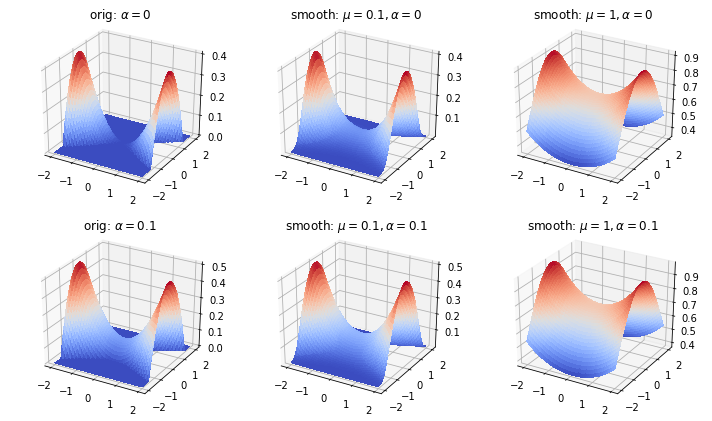
\includegraphics[width=\textwidth]{figures/triplet_viz.png}
  
  \caption{\label{fig:triplet_viz}This figure shows the triplet margin loss surface for a randomly generated 2-d triplet sample, with $\alpha = 0$ in the first row and $\alpha = 0.1$ in the second row. The leftmost plots show the original objective with no smoothing. The center plots show the smooth objective with $\mu=0.1$. The rightmost plots show the smooth objective with $\mu=1$. }
\end{figure}

\subsection{Smoothness analysis of $g(w)$}

We start by analyzing the formulation $f(w) = g(w) - h(w)$ using the methodology from \cite{khamaru_convergence_2018}. To use the theorem proven in that work, we need $g$ to be continuously differentiable and $M_g$-smooth, and we need $h$ to be continuous and convex. These properties are satisfied for the smooth reformulation from (\ref{eq:final_smooth_f}) and (\ref{eq:final_smooth_g}). Here, we will derive the value of $M_g$.

\begin{equation}
    \nabla g(w) 
    = \frac{ 2 \{ \exp((w^{\top}u)^2)uu^{\top} + \exp((w^{\top}v)^2)vv^{\top}  \} w}{ \exp((w^{\top}u)^2) + \exp((w^{\top}v)^2) }
\end{equation}

To find the Hessian, we break the gradient into two parts for use of the chain rule:

\begin{align*}
    \nabla (\nabla g(w) \; \textrm{top}) 
    &= 4 \{ \exp((w^{\top}u)^2)uu^{\top}ww^{\top}uu^{\top} + \exp((w^{\top}v)^2)vv^{\top}ww^{\top}vv^{\top} \} \\
    &= 4 \{ \exp((w^{\top}u)^2)(w^{\top}u)^2 uu^{\top} + \exp((w^{\top}v)^2)(w^{\top}v)^2 vv^{\top} \}
\end{align*}

\begin{align*}
    \nabla (\nabla g(w) \; \textrm{bot}) = \frac{ -2 \{ \exp((w^{\top}u)^2)uu^{\top} + \exp((w^{\top}v)^2)vv^{\top} \} w }{ \{ \exp((w^{\top}u)^2) + \exp((w^{\top}v)^2) \}^2 }
\end{align*}

Combining the parts:

\begin{align*}
    \nabla^2 g(w) &= 
    \frac{ 4 \{ \exp((w^{\top}u)^2)(w^{\top}u)^2 uu^{\top} + \exp((w^{\top}v)^2)(w^{\top}v)^2 vv^{\top} \} }{ \exp((w^{\top}u)^2) + \exp((w^{\top}v)^2)  } \\
    &- \frac{ 4 \{ \exp((w^{\top}u)^2)uu^{\top} + \exp((w^{\top}v)^2)vv^{\top}  \} ww^{\top} \{ \exp((w^{\top}u)^2)uu^{\top} + \exp((w^{\top}v)^2)vv^{\top}  \} }{ \{ \exp((w^{\top}u)^2) + \exp((w^{\top}v)^2) \}^2 }
\end{align*}

Re-arranging, we have:

\begin{align*}
    \nabla^2 g(w) &= 
    4 \left\{ \frac{  \exp((w^{\top}u)^2)(w^{\top}u)^2 uu^{\top}  }{ \exp((w^{\top}u)^2) + \exp((w^{\top}v)^2)  } +
    \frac{  \exp((w^{\top}v)^2)(w^{\top}v)^2 vv^{\top}  }{ \exp((w^{\top}u)^2) + \exp((w^{\top}v)^2)  } \right\} \\
    &- 4 \left\{
    \frac{  \exp((w^{\top}u)^2) uu^{\top}  }{ \exp((w^{\top}u)^2) + \exp((w^{\top}v)^2)  } + \frac{  \exp((w^{\top}v)^2) vv^{\top}  }{ \exp((w^{\top}u)^2) + \exp((w^{\top}v)^2)  } \right\}
    ww^{\top} \\
     & \left\{ \frac{  \exp((w^{\top}u)^2) uu^{\top}  }{ \exp((w^{\top}u)^2) + \exp((w^{\top}v)^2)  } + \frac{  \exp((w^{\top}v)^2) vv^{\top}  }{ \exp((w^{\top}u)^2) + \exp((w^{\top}v)^2)  }
     \right\}
\end{align*}

We can simplify further by using the substitution: 
\begin{align*}
p = \frac{\exp((w^{\top}u)^2)}{ \exp((w^{\top}u)^2) + \exp((w^{\top}v)^2) }
\end{align*}

Note that $0 < p < 1$, and:
\begin{align*}
1 - p = \frac{\exp((w^{\top}v)^2)}{ \exp((w^{\top}u)^2) + \exp((w^{\top}v)^2) }
\end{align*}

Plugging in to the Hessian expression:

\begin{align*}
    \nabla^2 g(w) &= 
    4 \{ p(w^{\top}u)^2 uu^{\top} + (1-p)(w^{\top}v)^2 vv^{\top} \} \\
    &- 4 \{ p uu^{\top} + (1-p) vv^{\top} \}ww^{\top}\{ p uu^{\top} + (1-p) vv^{\top} \} \\
    &= 4 p(w^{\top}u)^2 uu^{\top} + 4 (1-p)(w^{\top}v)^2 vv^{\top} \\
    &- 4 p^2 (w^{\top}u)^2 uu^{\top} - 4 (1-p)^2 (w^{\top}v)^2 vv^{\top} \\
    &- 8 p (1-p) (w^{\top}u)(w^{\top}v)(uv^{\top} + vu^{\top}) \\
    &= 4 p (1 - p) (w^{\top}u)^2 uu^{\top} + 4 p (1-p) (w^{\top}v)^2 vv^{\top} \\
    &- 8 p (1-p) (w^{\top}u)(w^{\top}v)(uv^{\top} + vu^{\top})
\end{align*}

Using $0 < p(1-p) \leq \frac{1}{4}$, we have, $\forall z \in \mathbb{R}^m$:

\begin{align*}
    z^{\top} \nabla^2 g(w) z &\leq
    z^{\top} \left\{ (w^{\top}u)^2 uu^{\top} + (w^{\top}v)^2 vv^{\top} - 2 (w^{\top}u)(w^{\top}v)(uv^{\top} + vu^{\top}) \right\} z \\
    &\leq \|z\|_2^2 \left\{ (w^{\top}u)^2 \|u\|_2^2 + (w^{\top}v)^2 \|v\|_2^2 + 4 \left| (w^{\top}u)(w^{\top}v)(u^{\top}v) \right| \right\} \\
    &\leq \|z\|_2^2 \|w\|_2^2 \left\{ \|u\|_2^4 + \|v\|_2^4 + 4 \|u\|_2^2 \|v\|_2^2 \right\}
\end{align*}

This gives us:

\begin{equation}
    \nabla^2 g(w) \preceq \|w\|_2^2 \left\{ \|u\|_2^4 + \|v\|_2^4 + 4 \|u\|_2^2 \|v\|_2^2 \right\} I_m
\end{equation}

Meaning that $g(w)$ is $M_g$-smooth, with $M_g = \|w\|_2^2 \left\{ \|u\|_2^4 + \|v\|_2^4 + 4 \|u\|_2^2 \|v\|_2^2 \right\}$.

%%%%%%%%%%%%%%%%%%%%%%%%%%%%%%%%%%%%%%%%%%%%%%%%%%%%%%%%%%%%%%%%%
\subsection{Smoothness analysis of $f(w)$}

In this section, we analyze the full function, instead of just $g(w)$, to see how the smoothness bound compares. Recall that $B = uu^\top - vv^\top$. We can rewrite the function in the softplus form by pushing all terms from the max into an exponential

\begin{equation}
\label{eq:f}
    f(w) = \log(\exp(w^{\top}Bw) + 1)
\end{equation}

\begin{equation}
    \nabla f(w) = \frac{2 \exp(w^{\top}Bw)Bw}{\exp(w^{\top}Bw) + 1}
\end{equation}

We can simplify the notation using the substitution

\begin{equation}
q = \frac{\exp(w^{\top}Bw)}{\exp(w^{\top}Bw) + 1}
\end{equation}

Applying this substitution, we have

\begin{equation}
\label{eq:grad_f}
    \nabla f(w) = 2qBw
\end{equation}

To find the Hessian, we break the gradient into two parts for use of the chain rule:

\begin{align*}
    \nabla (\nabla f(w) \; \textrm{top}) = 4 \exp(w^{\top}Bw)Bww^{\top}B  + 2 \exp(w^{\top}Bw)B
\end{align*}

\begin{align*}
    \nabla (\nabla f(w) \; \textrm{bot}) = \frac{-2 \exp(w^{\top}Bw)B}{\exp(w^{\top}Bw) + 1}
\end{align*}

Combining the parts:

\begin{align*}
    \nabla^2 f(w) = \frac{4 \exp(w^{\top}Bw)B(ww^{\top}B + \frac{1}{2}I_m)}{\exp(w^{\top}Bw) + 1} - \frac{4 \{\exp(w^{\top}Bw)\}^2 Bww^{\top}B }{\{\exp(w^{\top}Bw) + 1\}^2}
\end{align*}

Using this substitution of $q$,  we have:
\begin{equation}
    \nabla^2 f(w) = 4q(1-q)Bww^{\top}B + 2qB
\end{equation}

Noting that $0 < q < 1$ and $0 < q^2 \leq \frac{1}{4}$ we have, $\forall z \in \mathbb{R}^m$:

\begin{align*}
z^{\top} \nabla^2 f(w) z 
&= 4q(1-q) z^{\top} Bww^{\top}B z + 2q z^{\top} B z \\
&< z^{\top} Bww^{\top}B z + 2 z^{\top} B z \\
&\leq \|z\|_2^2 \|w\|_2^2 \lambda_{\max} (B)^2 + 2 \|z\|_2^2 \lambda_{\max} (B) \\
&= \|z\|_2^2 ( \|w\|_2^2 \lambda_{\max} (B)^2 + 2 \lambda_{\max} (B) ) 
\end{align*}

This gives us:

\begin{equation}
    \nabla^2 f(w) \prec ( \|w\|_2^2 \lambda_{\max} (B)^2 + 2 \lambda_{\max} (B)) I_m
\end{equation}

Meaning that $f(w)$ is $M_f$-smooth, with $M_f = \|w\|_2^2 \lambda_{\max} (B)^2 + 2 \lambda_{\max} (B)$. We note that this smoothness bound is usually better than the one achieved in the previous section when analyzing only $g(w)$.

We also note that since we have shown the function is twice continuously differentiable and $M_f$-smooth, the set of initial points for which gradient descent converges to a strict saddle point has measure zero, as proven in \cite{lee_gradient_2016}.

\subsection{Gradient descent analysis of $f(w)$}
\label{sec:grad_descent}

We analyze the standard gradient step

\begin{equation}
    w^{t+1} = w^t - \eta \nabla f(w^t)
\end{equation}

We would like to show that the following descent condition holds for some $\eta > 0, c < 0$

\begin{equation}
\label{eq:descent_condition}
    f(w^{t+1}) \leq f(w^t) + c
\end{equation}

This property is not guaranteed in general for a difference of convex functions, and we cannot rely on properties of convexity that would typically be applied. Fortunately, this function has special structure as we will show in the following derivation.

\begin{equation}
    f(w^{t+1}) = f(w^t - \eta \nabla f(w^t)) 
\end{equation}

Using $\nabla f(w))$ from Eq. (\ref{eq:grad_f}) , we have

\begin{align*}
    w - \eta \nabla f(w) &= w - 2qBw \\
    &= (I_m - 2qB)w
\end{align*}

Applying this term to $f$ from (\ref{eq:f}), we get

\begin{equation}
\begin{split}
    f(w^t - \eta \nabla f(w^t)) 
    &= \log(\exp(w^{\top}(I_m - 2 \eta qB)B(I_d - 2 \eta qB)w) + 1) \\
    &= \log(\exp(w^{\top}Bw + w^{\top} ( 4 \eta^2 q^2 B^3 - 4 \eta q B^2)w) + 1)
\end{split}
\end{equation}

Let $b_\eta = w^{\top} ( 4 \eta^2 q^2 B^3 - 4 \eta q B^2)w$. Making this substitution, we have

\begin{equation}
\begin{split}
    f(w^t - \eta \nabla f(w^t)) 
    &= \log(\exp(w^{\top}Bw + b_\eta ) + 1) \\
    &= \log(\exp(w^{\top}Bw)\exp(b_\eta ) + 1)
\end{split}
\end{equation}

Examining the desired descent condition from (\ref{eq:descent_condition}), we want to find some $c < 0$ such that

\begin{align*}
    f(w^{t+1}) - f(w^t) \leq c
\end{align*}

Substituting in, we find that

\begin{align*}
    f(w^{t+1}) - f(w^t) &= 
    \log(\exp(w^{\top}Bw)\exp(b_\eta ) + 1) - \log(\exp(w^{\top}Bw) + 1) \\
    &= \log \left\{ \frac{\exp(w^{\top}Bw)\exp(b_\eta ) + 1}{\exp(w^{\top}Bw) + 1} \right\} \\
    &= \log( q \exp(b_\eta ) + (1 - q))
\end{align*}

Therefore, we must select $c < \log( q \exp(b_\eta ) + (1 - q))$ to satisfy the descent condition. In particular, this form shows that the descent condition holds for $b_\eta < 0$.

\subsection{Selecting the step size $\eta$}

Since we have that $f(w^{t+1}) < f(w^t) + c, \; c < 0$ we would like to select the step size $\eta$ such that $c$ is minimized at each step. Using the direct line search approach, we attempt to solve the following optimization problem:

\begin{equation}
    c^* = \min_{\eta} \log( q \exp(b_\eta ) + (1 - q))
\end{equation}

In terms of $\eta$, we want to find

\begin{equation}
\label{eq:eta_opt}
\begin{split}
    \eta^* &= \argmin_{\eta} \log( q \exp(b_\eta ) + (1 - q)) \\
    &= \argmin_{\eta} b_\eta \\
    &= \argmin_{\eta} w^{\top} ( 4 \eta^2 q^2 B^3 - 4 \eta q B^2)w
\end{split}
\end{equation}

Although the function is not convex in $\eta$, we can search for a first order critical point.

\begin{align*}
\nabla_{\eta} w^{\top} ( 4 \eta^2 q^2 B^3 - 4 \eta q B^2)w 
&= 8 \eta q^2 w^{\top} B^3 w - 4 q w^{\top} B^2 w = 0 \\
&\implies 2 \eta q w^{\top} B^3 w = w^{\top} B^2 w \\
&\implies \eta = \frac{w^{\top} B^2 w}{2 q w^{\top} B^3 w} \\ 
&\implies \eta \leq \frac{1}{2q\lambda_{\max}(B)} \\
&\implies \hat{\eta} = \frac{1}{2q\lambda_{\max}(B)}
\end{align*}

Although we can't show $\hat{\eta}$ minimizes $b_{\eta}$, we can show it is a good choice by examining the eigenvalues of $b_{\hat{\eta}}$. Let $B = U^{\top} \Lambda U$ be the spectral decomposition of $B$. Then we have

\begin{align*}
    b_{\hat{\eta}} &= w^{\top} ( 4 \hat{\eta}^2 q^2 B^3 - 4 \hat{\eta} q B^2)w \\
    &= w^{\top} \left( \frac{B^3}{\lambda_{\max}(B)^2} - \frac{2 B^2}{\lambda_{\max}(B)} \right) w \\
    &= w^{\top} U^{\top} \left( \frac{\Lambda^3}{\lambda_{\max}(B)^2} - \frac{2 \Lambda^2}{\lambda_{\max}(B)} \right) Uw
\end{align*}

In this form, we can see that all the eigenvalues in the inner term must be $\leq 0$. Although this choice of $\eta$ guarantees descent, there is not an easy way to isolate terms so we can use the condition for convergence analysis. The strongest claim we can make is that $b_{\hat{\eta}} \leq 0$.

Comparing to the smoothness of $w^{\top}Bw = \lambda_{\max}(B) = M$ from Section \ref{sec:composite_smoothness}, $\frac{1}{M}$ is very close to the stepsize $\hat{\eta}$, suggesting that the function behavior is dominated by the underlying quadratic.

In Appendix \ref{app:grad_descent}, we compare this this choice of stepsize to ones derived from smoothness in the previous sections, for a simple gradient descent experiment.

% Solve two cases: one where B is PSD, the other where it isn't
% Recall that $B \nsucceq 0$, which means that problem (\ref{eq:eta_opt}) is not convex. We will show that a good choice of $\eta$ is $\eta = \frac{1}{\|B\|_2}$.

% \begin{align*}
%     b_\eta &= w^{\top} ( 4 \eta^2 q^2 B^3 - 4 \eta q B^2)w \\
%     &= \frac{4 q^2 w^{\top} B^3 w}{\|B\|_2^2} - \frac{4 q w^{\top} B^2 w}{\|B\|_2} \\
%     &\leq \frac{4 q^2 \|B\|_2^3}{\|B\|_2^2} - \frac{4 q \|B\|_2^2 }{\|B\|_2} \\
%     &= 4 q (q-1) \|B\|_2 \\
%     &\implies -\|B\|_2 \leq 4 q (q-1) \|B\|_2 \leq 0
% \end{align*}

% The last step using $-\frac{1}{4} \leq q (q-1) \leq 0$. Since the given choice of $\eta$ is the largest valid choice which guarantees $b_\eta \leq 0$, it is optimal.

\subsection{Coarse bound on the iterate}

Using the stepsize $\eta = \hat{\eta}$

\begin{align*}
    w^{t+1} = w^t - \hat{\eta} \nabla f(w^t)
    &= (I_m - 2q \hat{\eta} B)w^t \\
    &= \left( I_m - \frac{B}{\lambda_{\max}(B)} \right) w^t \\
    &= \left( I_m - \frac{B}{\lambda_{\max}(B)} \right)^t w^1
\end{align*}

Taking the norm of both sides, we have

\begin{align*}
    \|w^{t+1}\|_2 &= \left\|\left( I_m - \frac{B}{\lambda_{\max}(B)} \right)^t w^1 \right\|_2 \\
    &\leq \left\|\left( I_m - \frac{B}{\lambda_{\max}(B)} \right)^t \right\|_F \|w^1\|_2
\end{align*}

Since there is no guarantee on what the norm of some $w^*$ should be, this bound is not very useful in practice.

\subsection{Convergence of the squared gradient norm}

%In \cite{khamaru_convergence_2018}, the following bound is given on the average squared gradient norm, with $\eta \in (0, \frac{1}{M_g}]$

Choosing a stepsize of $\eta = \frac{1}{M_f}$, we have the standard bound

\begin{equation}
    \sqrt{\frac{1}{T} \sum_{t=1}^{T} \| \nabla f(w^t) \|_2^2} \leq \sqrt{\frac{2 M_f (f(w^1) - f(w^*))}{T}}
\end{equation}

However, since both of our derived smoothness terms depend on the iterate, we cannot assume this bound. So we will instead utilize our descent condition from Section \label{sec:grad_descent}.

We have

\begin{equation}
    \| \nabla f(w) \|_2^2 = 4 q^2 w^{\top} B^2 w
\end{equation}

From Section \ref{sec:grad_descent}, choosing $\eta = \frac{1}{\lambda_{\max}(B)}$, we have

\begin{align*}
    b_\eta &= w^{\top} ( 4 \eta^2 q^2 B^3 - 4 \eta q B^2)w \\
    &= \frac{\nabla f(w)^{\top} B \nabla f(w)^{\top}}{\lambda_{\max}(B)^2} - \frac{\| \nabla f(w) \|_2^2}{q \lambda_{\max}(B)} \\
    &\leq \frac{ \lambda_{\max}(B) \| \nabla f(w) \|_2^2}{\lambda_{\max}(B)^2} - \frac{\| \nabla f(w) \|_2^2}{q \lambda_{\max}(B)}\\
    &= \frac{(q-1) \| \nabla f(w) \|_2^2}{q \lambda_{\max}(B)}
\end{align*}

This gives us

\begin{align*}
    f(w^{t+1}) - f(w^t) &\leq \log( q \exp(b_\eta ) + (1 - q)) \\
    &= \log \left( q \exp \left( \frac{(q-1) \| \nabla f(w^t) \|_2^2}{q \lambda_{\max}(B)} \right) + (1 - q) \right) \\
    &\implies \log \left( q \exp \left( \frac{(1-q) \| \nabla f(w^t) \|_2^2}{q \lambda_{\max}(B)} \right) + (1-q) \right) \leq f(w^t) - f(w^{t+1}) 
\end{align*}

Finally, we have

\begin{align*}
    \sum_{t=1}^{T} \log \left( q \exp \left( \frac{(1-q) \| \nabla f(w^t) \|_2^2}{q \lambda_{\max}(B)} \right) + (1-q) \right) &\leq f(w^1) - f(w^{T}) \\
    &\leq f(w^1) - f(w^{*})
\end{align*}

The term inside the log is always positive, and $q \exp(.) + (1-q) = 1$ if and only if $\exp(.) = 0$, which can occur only if $\| \nabla f(w^t) \|_2^2 = 0$, since $0 < q < 1$. Therefore, we can conclude that $\| \nabla f(w^t) \|_2^2 \rightarrow 0$. Unfortunately, it is difficult to compare this bound against the standard smoothness bound, since the norm gradient term can't be trivially freed from the logs and exponentials.

Another approach to this analysis could be to use the smoothness term directly for the standard smoothness descent condition

\begin{equation}
    f(w^{t+1}) \leq f(w^t) - \frac{1}{2M_f}\| \nabla f(w^t) \|_2^2
\end{equation}

We could attempt to free the iterate term from the smoothness. An easy way to do that would be to restrict $\|w\|_2^2 \leq 1$.

\subsection{Convergence of the function value}

Using the gradient update, we have

\begin{align*}
    w^{t+1\top}Bw^{t+1} &\leq w^{t\top}Bw^{t} + b_\eta \\
    &\leq w^{1\top}Bw^{1} + \sum_{k=1}^{t+1} b_\eta^k \\
    &\implies \log( \exp(w^{t+1\top}Bw^{t+1}) + 1) \leq \log( \exp(w^{1\top}Bw^{1} + \sum_{k=1}^{t+1} b_\eta^k) + 1) \\
    &\implies f(w^{t+1}) \leq \log( \exp(w^{1\top}Bw^{1} + \sum_{k=1}^{t+1} b_\eta^k) + 1)
\end{align*}

Now we can say

\begin{align*}
    f(w^{t+1}) - f^* &\leq \log( \exp(w^{1\top}Bw^{1} + \sum_{k=1}^{t+1} b_\eta^k) + 1) - f^* \\
    &= \log( \exp(w^{1\top}Bw^{1} + \sum_{k=1}^{t+1} b_\eta^k) + 1) - \log( \exp(w^{*\top}Bw^{*}) + 1) \\
    &= \log \left( \frac{\exp(w^{1\top}Bw^{1} + \sum_{k=1}^{t+1} b_\eta^k) + 1}{\exp(w^{*\top}Bw^{*}) + 1} \right) \\
    &\leq \log \left( \frac{\exp(w^{1\top}Bw^{1} + \sum_{k=1}^{t+1} b_\eta^k)}{\exp(w^{*\top}Bw^{*})} + 1 \right) \\
    &= \log \left( \exp \left(w^{1\top}Bw^{1} - w^{*\top}Bw^{*} + \sum_{k=1}^{t+1} b_\eta^k \right) + 1 \right)
\end{align*}

Simplifying further appears to be nontrivial, and we can't make a claim about the iteration complexity without somehow freeing the iteration count from the summation term.

\subsection{Experiments}

%\subsection{Extension to case with $\mu \neq 1$ and $\alpha > 0$}

%\subsection{Extension to case with $m > 1$}

%\subsection{Analysis with bias term}

%To simplify analysis of gradient methods, we will concatenate $A$ and $b$ and append a $1$ to $x$: $\tilde{A} = [A, b]$, $\tilde{x}^\top = [x^\top, 1]$. Now we have $f(\tilde{A}; \tilde{x}) = \tilde{A} \tilde{x}$, $\tilde{A} \in \mathbb{R}^{d \times m+1}$.

% \subsection{Analysis of Gradient Method}

% We analyze this formulation using the methodology from \cite{khamaru_convergence_2018}. To use the theorem proven in that work, we need $g$ to be continuously differentiable and $M_g$-smooth, and we need $h$ to be continuous and convex. These properties are satisfied for affine choice of $f$ in Problem (\ref{eq:smooth_dc}).

% Since $h_i(\theta)$ is differentiable for our case, we can use a regular gradient step and achieve the convergence bound for Algorithm 1 in \cite{khamaru_convergence_2018}. Not sure if it is necessary to constrict $\theta \in \mathcal{C}$ as in \cite{khamaru_convergence_2018}, but this can be done if necessary.

% $A = w = 0$ does not minimize this function because of the margin parameter $\alpha$. As for finding a closed form solution, we can see if it is clear from computing the gradient.

%\subsubsection{Does this smooth version allow for triplets which violate the original objective? If so, can this violation be quantified?}

\section{Conclusion}

\subsection{Discussion}

In this work, we show that the triplet margin loss function can be reformulated as a difference of convex functions, and that a reasonable smooth approximation can be formulated with the LogSumExp function. We show that this function is smooth, and give an upper bound for the smoothness which is dependent on the iterate. Then, we show that a descent condition not directly related to the smoothness holds for the gradient descent algorithm, given the right choice of stepsize. Finally, we attempt a gradient descent convergence analysis for the iterate, the squared gradient norm, and the function value. While none of the convergence bounds achieved are very useful, they provide insight into the structure of the function, and lay a nice foundation for future work.

One conclusion from this effort is that the condition of convexity cannot be trivially replaced just by knowing the function structure. Still, by showing that the triplet function is smooth, and that it satisfies a descent condition separate from its smoothness, we have shown that the function is more relaxed than the conditions imposed from \cite{khamaru_convergence_2018}. Further analysis should yield a faster rate than the bound on the norm squared gradient achieved from smoothness.

\subsection{Future Work}

There are several extensions that we would like to perform on this analysis. First, we would like to repeat the analysis for $\alpha > 0$ and $\mu \neq 1$. Second we would like to analyze the multi-sample case ($n > 1$). Third we would like to study the case where $d > 1$. Fourth, we would like to add a learnable bias term to the analysis. Finally, we would like to study the stochastic case, so that this work can be applied in practice for empirical risk minimization, given randomly sampled data. These insights can be imported back to the deep learning setting to have a more principled understanding of optimization in that context.

In addition, we would like to conduct a similar analysis for the contrastive loss function posed in \cite{hadsell_dimensionality_2006}, which optimizes over pairs of samples instead of triplets. This loss function can be reformulated as a triplet loss by considering two pairs, and is also a DC function that can be smoothed with LogSumExp. We would like to compare convergence bounds, and then conduct an empirical analysis, to determine which objective generalizes better to new data.

We would also like to compare the triplet loss to the soft margin loss and logistic loss for the support vector machine (SVM). It would be interesting to study the learned hyperplane boundary from $w$, and see how the models compare in terms of generalization.

% \subsection{Previously wanted next steps}

% \begin{itemize}
%   \item Trying different gradient methods
%   \item Use Nesterov momentum as in the Princeton slides
%   \item Analyzing stochastic gradient method for the problem
%   \item Attempting to analyze the non-smoothed problem
%   \item Empirical analysis using toy separable data with two classes
%   \item Compare empirical behavior of gradient methods for the relaxed problem vs. the original problem
%   \item Compare nearest neighbors performance for difference constraints on the weight space, C
% \end{itemize}

\bibliography{references}

%\appendix

\begin{appendices}
\section{Gradient Descent Experiment}
\label{app:grad_descent}

\begin{figure}[!h]
  \centering
  %\fbox{\rule[-.5cm]{0cm}{4cm} \rule[-.5cm]{4cm}{0cm}}
  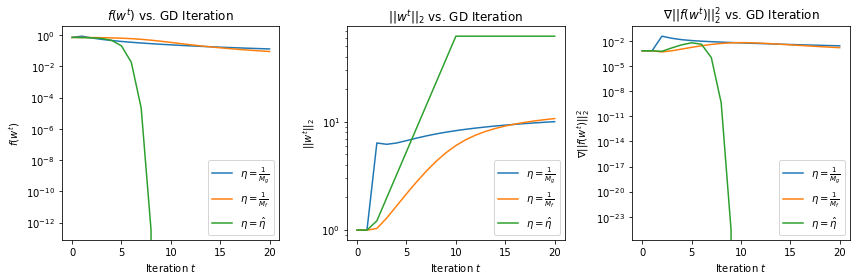
\includegraphics[width=\textwidth]{figures/triplet_descent.png}
  
  \caption{\label{fig:triplet_descent}This figure gradient descent on the triplet margin loss for a randomly generated 2-d triplet sample, with $\alpha=0, \mu=1$. The three plots correspond to the function value, norm of the iterate, and norm squared of the gradient respectively. Each plot has three stepsizes, chosen based on the bounds for $M_g$, $M_f$, and $\hat{\eta}$. Notice that the function value descends monotonically for all choices of $\eta$, but descends much faster for $\eta = \hat{\eta}$ (appears to be quadratic in log space). Also, notice that the norm squared of the gradient increases before decreasing, which can be explained by the saddle structure of the loss surface.}
\end{figure}

%\section{Some More Notation}
\end{appendices}

\end{document}
\grid
\grid